\cleardoublepage
\chapter{Diseño e implementación}
\label{chap:design_implement}


En este capítulo se realiza una descripción detallada sobre el diseño y la implementación del presente Proyecto de Fin de Carrera.\\


\section{Modelo de desarrollo} 
\label{subsec:modelo_desarrollo}

El desarrollo de un proyecto de software libre implica una sucesión de tareas entre el momento que se tiene una idea para resolver un problema o necesidad, y el producto u servicio final que lo satisface. Este metodología nos marca como se suceden las diferentes tareas y actividades dentro del proyecto.\\


Durante el desarrollo de este proyecto hemos seguido un modelo que se asemeja al modelo de desarrollo iterativo y creciente, o incremental.  En este proceso creamos una primera versión del sistema, funcional, con el que se pueda interactuar y nos dé realimentación para las sucesivas iteraciones.\\


El modelo incremental, a priori, nos proporciona las siguientes ventajas:\\

\begin{itemize}
\item Al desarrollar sistemas más pequeños con subconjuntos de los requerimientos o funcionalidades, reducimos el riesgo asociado a realizar el desarrollo en bloque del sistema completo.\\

\item Al desarrollarse progresivamente parte de las funcionalidades, se puede evaluar mejor si los requerimientos de los siguientes incrementos son correctos o hay que adaptarlos a la realidad.\\

\item En caso de errores o problemas, generalmente afecta a la última interacción y no a todo el conjunto, volviendo al incremento previo en el peor caso.\\

\item En el caso de este proyecto, me permitía avanzar paso a paso en el desarrollo del sistema mientras iba adquiriendo la experiencia necesaria para desarrollar mejor o redefinir mejor los siguientes incrementos.\\
\end{itemize}


Además, este modelo tiene gran similitud con el modelo que nuestro profesor adoptaba para la evolución de las prácticas de sus asignaturas durante el curso. Las cuales empezaban con prácticas sencillas o introductorias, a las que se le iban añadiendo elementos, funcionalidades y complejidad, hasta llegar a la práctica final, que mirando retrospectivamente, había sido una sucesión de incrementos a partir de una estructura inicial que se había establecido prácticas atrás.\\


Para observar esto último, en el caso de este proyecto, disponíamos de algunas muestras de grupos de repositorios de actividades en diferentes etapas del trimestre, los cuales, por ejemplo, podemos clasificar según a la exigencia que nos va a suponer para nuestro sistema corrector Misture.\\

\textbf{GRUPO 1}


\begin{itemize}
\item Actividades en las semanas iniciales del trimestre o introductorias.\\

\item Pequeños proyectos con poca cantidad de código y elementos que exige un análisis de código Python más simple.\\

\item Salidas de ejecuciones más sencillas: cierto fichero con un contenido concreto, cadenas cortas de valores concretos, etc.\\

\item Puede requerir algunas comprobaciones sencillas sobre ficheros o documentos XML\\

\item Por el momento, al alumno se le está introduciendo en temas de calidad y estilo de código, y es suficiente con contar los errores e imprimirle al alumno que errores comete, que significan y en que código se produce.\\
\end{itemize}


\textbf{GRUPO 2:}


\begin{itemize}
\item Actividades de etapas avanzadas del trimestre o de materias de mayor nivel.\\

\item Escenarios de mayor cantidad y complejidad de código fuente: aplicaciones cliente-servidor con lógicas complejas, desarrollo de aplicaciones sobre frameworks que conllevan mayor complejidad en la estructura del proyecto entregado, etc.\\

\item Análisis de código Python más complejo y rico.\\

\item La propia prueba de ejecución de la aplicación o aplicaciones se vuelve más difícil, y no nos sirven de igual forma cierto tipo de pruebas de ejecución en unos escenarios u otros.\\

\item En este punto, es interesante obtener información más rica sobre estilo y calidad de código y errores, para poder luego analizarse o reportarse asociado a su fichero fuente, u observar la evolución temporal de la calidad y errores de nuestro código.
\end{itemize}


De acuerdo al modelo de desarrollo descrito, en una fase inicial, recogimos de forma general los requerimientos del sistema completo, en base a la descripción del problema y las experiencias previas descritas en el Capítulo \ref{chap:objetivos} de la presente memoria.\\


Una vez se disponen de los requisitos, se crea una versión inicial funcional, que comenzamos con un modulo principal, que disponía de las configuraciones básicas para obtener los repositorios y conocer los requisitos básicos como que ficheros deben entregarse.\\


A partir de ese versión inicial, se fueron añadiendo los módulos con los diferentes grupos de funcionalidades, los cuáles íbamos probando frente a las muestras de los repositorios de alumnos de las que dispusimos. Es decir, realizábamos incremento para agregar funcionalidad básica de análisis de código Python, posteriormente otra iteración para la extracción de información básica del repositorio git, etc.\\


Para simplificar la explicación del diseño de Misture, vamos a reducir la explicación de todo el proceso al detalle de dos estados, que vamos a denominar iteración 1 e iteración 2, que realmente componen una sucesión de incrementos que llevaron a esos dos estados del proyecto.\\


Esta división, asimismo, tiene también como justificación el hecho de que el estado descrito en la primera iteración es más próxima a las actividades caracterizadas del grupo 1 descrito anteriormente, y la iteración 2 recoge un estado más cercano a resolver las necesidades de las actividades descritas en el grupo 2.

\section{ITERACION 1:}

Vamos a describir el diseño de los diferentes módulos que componen este primera sucesión de incrementos. En la figura de abajo se muestra un esquema de flujo de está primera ``versión'' de Misture.\\


En este diseño, para el almacenamiento y tratamiento de todos los datos extraídos en los diferentes análisis, se emplearon ficheros para las transacciones entre las utilidades externas y para generar logs de errores e imprimir el reporte final ordenado, así como estructuras dinámicas como listas y diccionarios y una jerarquía de clases Python que modelaban los diferentes objetos y las relaciones entre ellos que identificábamos en este escenario, tales como actividad, alumnos, repositorios, ficheros, elementos de código, estadística, error de estilo, etc.\\


Esta jerarquía, era una primera versión del modelo usado en la iteración 2 y que se detalla posteriormente en en el apartado ``DISEÑO DE BBDD''.

\subsection{MÓDULO PRINCIPAL}

En el modulo MainAnaly, se establece la configuración básica de la actividad a corregir, como la ubicación de los repositorios asociados a los logines de alumnos, los nombres de los ficheros y códigos fuentes que deben estar en el repositorio, así como las tuplas con las llamadas a los programas del alumno y las salida que debe obtener el programa en caso de funcionar correctamente según la especificación de la actividad.\\


Este módulo, también se encarga de cargar esta configuración en la jerarquía de clases del escenario e inicializar los logs para la actividad y establecer una ubicación para los reportes individualizados.\\


A continuación, realiza las diferentes llamadas a los módulos de análisis, a los que les proporciona como parámetros los objetos adecuados del escenario -repositorio, fichero, etc- y recoge los resultados del análisis, asociándolos al objeto del mundo Misture correspondiente.

\subsection{MÓDULO DE ANÁLISIS DE CÓDIGO PYTHON}

Este módulo, llamado \textit{PyfichAnaly}, implementa la funcionalidad relativa a la identificación de los ficheros presentes en el repositorio del proyecto, en función de una lista predefinida de ficheros.\\


Como novedad, en este análisis se detecta si al alumno le falta alguno de los ficheros requeridos por la práctica, y a través de una pequeña heurística intenta deducir si hay otros ficheros que de nombre similar que puedan serlo.\\


Esta heurística, se basa en el algoritmo de Levenhstein, es un algoritmo que tiene la capacidad medir la cantidad de operaciones de inserción, borrado o cambio de caracteres que hay entre dos cadenas de texto.\\


Por tanto, en caso de que se encuentren archivos huérfanos en la lista de ficheros requeridos y en el repositorio, y siempre que no supere un umbral, se entiende que el fichero con la menor distancia de Levenhstein es aquel que nos falta, y por tanto, se renombra y se prosiguen los análisis.\\


Una vez identificados los ficheros disponibles, se identifican los que son ficheros fuente Python, y se llama a la clase \textbf{PyModuleCont}, que analiza el código fuente del fichero a través de patrones regulares y funciones de las librería re de Python, cuya muestra se adjunta en la figura inferior.\\


De dicho análisis, asociamos al fichero Python los elementos clase, método y función que contengan, junto a su nombres.\\


\begin{figure}[H]
   \centering
   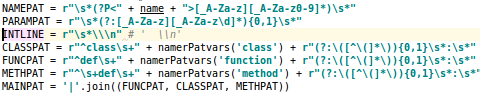
\includegraphics[width=16cm]{img/Selection_022_pyanaly_regex}
   \caption{regex utilizados para identificar elementos de código y su nombre}
   \label{figura:regex}
\end{figure}

\subsection{MÓDULO DE ANÁLISIS DE CALIDAD DEL CÓDIGO}

En el módulo \textbf{CodeAnaly.py}, se implementa la funcionalidad de análisis de calidad del código, que en esta iteración del desarrollo de Misture, se realiza con ayuda de las utilidades \textit{Pep8}, para el análisis de estilo, y \textit{Pylint}, para el análisis estático del código.\\


El procedimiento de análisis de estilo, se implementa en la clase \textbf{Pep8Analy}, es una clase con los atributos necesarios para almacenar los errores de estilo, ficheros en que se producen, y estadísticas de los errores.\\


\textbf{Pep8Analy}  recibe como configuración las rutas de los ficheros python a analizar, y los códigos de error que no deben ser tenidos en cuenta para este análisis. Y se inicializa invocando a la utilidad \textit{pep8} como se indica abajo, para recopilar los errores detectados y un sumario de estadísticas.

\begin{verbatim}
pep8 --repeat --show-source –ignore=<codigos_error>
<ruta1_py ruta2_py...>

pep8 -q --statistics <ruta_py1 ruta_py2...>
\end{verbatim}


Por otra parte, también se implementa una clase \textbf{PylintAnaly}, que con un funcionamiento semejante al de \textit{Pep8Analy}, extrae y guarda de forma estructurada los errores \textit{Pylint} y la nota de calidad del código obtenidas de la utilidad llamada de la siguiente manera.

\begin{verbatim}
pylint –disable=<codigos_error> <ruta_py1 ruta_py2 ...>
\end{verbatim}


\subsection{MÓDULO DE PRUEBAS DE EJECUCIÓN}

\begin{figure}[H]
   \centering
   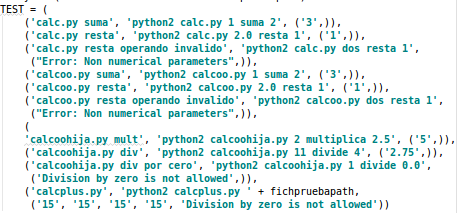
\includegraphics[width=16cm]{img/Selection_024_testcodigo}
   \caption{Tuplas con la batería de pruebas para el módulo de pruebas}
   \label{figura:testcodigo}
\end{figure}

La clase \textbf{testPr} itera sobre cada una de las tuplas de prueba, ejecuta la prueba, e invoca a un pequeño módulo denominado \textbf{OutputAnaly}, que chequea a través de funciones de texto y de la librería \textit{re} de Python que la salida recogida es compatible con la salida esperada, permitiendo cierta incertidumbre introducida por cambios en la capitalización, introducción de separadores o caracteres blancos, etc.

\subsection{MÓDULO DE ANÁLISIS DE GIT}


En esta versión de Misture, se implementa un análisis sencillo de repositorio Git. Dicho análisis, se realiza a través del parseo de la salida de la siguiente llamada a git.
\begin{verbatim}
git log <ruta_repo_alumno>
\end{verbatim}
A la salida del \textit{log}, se le extraen mediante funciones de la librería re de Python y los patrones adecuados los datos del autor del commit.\\


Asimismo, podemos proporcionarle un listado de palabras o raíces de palabras que consideramos clave en los \textit{commits} de la actividad que corregimos por su significancia, obteniendo  del análisis el número de apariciones, y en consecuencia, una medida sobre si el alumno etiqueta los \textit{commits} con buen criterio.


\begin{figure}[H]
   \centering
   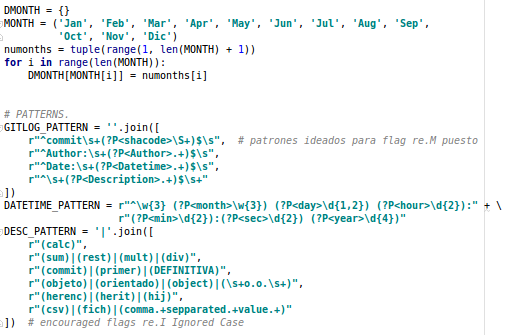
\includegraphics[width=16cm]{img/Selection_025_gitlog_patterns}
   \caption{Regex utilizados para el análisis del log}
   \label{figura:reg_analisis_log}
\end{figure}

\subsection{MÓDULO DE COMUNICACIÓN}

Con el objetivo de dotar de nuevas funcionalidades a Misture y automatizando y reduciendo el tiempo necesario para todas las tareas. Se implemento una funcionalidad con el objetivo de poder comunicar masivamente el resultado de las prácticas. Esta funcionalidad la implementamos en el módulo \textbf{mailing}.\\

En dicho módulo, a través la funcionalidad de las librerías \textit{smtplib} y \textit{email} de Python, o la API del servicio de emailing \textit{SendGrid}, hay implementaciones para realizar el envío automatizado de los reportes, siempre que se proporcionen las credenciales de acceso.


\section{DISEÑO DE BBDD} 
\label{subsec:bbdd}

En la versión más reciente de Misture, se optó por emplear el sistema de base de datos MongoDB, con bases de datos no relacionales, sin esquema, o mejor dicho, de esquema dinámico.\\


La elección de MongoDB para almacenar todos los datos obtenidos de los análisis de los repositorios, pruebas, y comprobaciones de código, en principio facilita y nos permite ser más ágiles durante el desarrollo y prueba de los diferentes módulos y funcionalidades. Por una parte por no trabajar con un esquema rígido y por otra porque MongoDB encaja muy bien con los tipos de datos nativos de Python – objetos, listas, diccionarios-.\\


Adicionalmente, buscamos una librería ODM -Object Document Mapper- para MongoDB en Python, permitiéndonos operar con la BBDD como si fuera un objeto, facilitando aún más nuestra labor. En un primer momento se eligió \textbf{mongoengine}, aunque al final en Misture hemos utilizado \textbf{pymodm}.\\


Se debe recordar, que la estructura y validaciones de los campos definidos en las clases documento del ODM que representan los documentos de las colecciones de MongoDB son transparentes al propio MongoDB, se producen en el lado de la aplicación a través del ODM.\\


A continuación, vamos a enumerar los diferentes documentos considerados para poder llevar a cabo la funcionalidad básica de Misture.\\


[FIGURA XX: Representación de BBDD incluida en Misture]


\textbf{LogError} es la clase del documento donde se vuelcan los errores controlados de la ejecución de Misture.
\begin{itemize}
\item descripcion
\item accion
\item traza
\item fecha
\item actividad: referencia a \textbf{Actividad}
\item correccion: referencia a \textbf{Correccion}
\end{itemize}


\textbf{UsuarioMisture} representa a un usuario del sistema Misture.
\begin{itemize}
\item login
\item email
\item rol
\item date
\end{itemize}


\textbf{Corrector} es la clase heredera de \textbf{UsuarioMisture} que modela las particularidades del usuario corrector.
\begin{itemize}
\item actividades: referencia a \textbf{Actividad}
\item rol
\item superrol
\end{itemize}


\textbf{Desarrollador} es la subclasde de \textbf{UsuarioMisture} que representa al desarrollador.
\begin{itemize}
\item emails
\item rol
\end{itemize}


\textbf{DirectoriosActividad} representan las rutas particulares donde se ubicarían los ficheros de la actividad a corregir.
\begin{itemize}
\item pbase
\item pentrega
\item presultados
\item perrores
\item ptest
\item ppruebas
\end{itemize}


\textbf{Actividad} es la clase que representa una actividad, con sus datos básicos para ser corregida.
\begin{itemize}
\item descripcion
\item corrector -> referencia a \textbf{Corrector}
\item desarrolladores -> referencia a \textbf{Desarrollador}
\item entregas -> documento Entrega
\item directorios -> documento \textbf{DirectoriosActividad}
\item ficheros\_entrega
\end{itemize}


\textbf{Correccion} es la clase que representa a la ejecución de una corrección de una entrega de un alumno.
\begin{itemize}
\item fecha
\item actividad -> referencia a \textbf{Actividad}
\item desarrollador -> referencia a \textbf{Desarrollador}
\item desarrolladores -> referencia a \textbf{Desarrollador}
\item gitanaly -> documento \textbf{GitAnaly}
\end{itemize}


\textbf{Entrega} es la clase que modela los elementos necesarios para emprender la corrección de la actividad de un alumno particular.
\begin{itemize}
\item actividad: referencia a \textbf{Actividad}
\item desarrollador: referencia a \textbf{Desarrollador}
\item modo
\item ubicacion
\item correccion: referencia al documento corrección.
\end{itemize}


\textbf{Prueba} modela una prueba de caja negra.
\begin{itemize}
\item correccion: referencia a \textbf{Correccion}
\item llamadas\_ord
\item outputs
\end{itemize}


\textbf{Udfile} representa a un fichero o directorio de una entrega.
\begin{itemize}
\item correccion -> referencia a \textbf{Correccion}
\item pathrel
\item nombre
\item tipo
\item hijos -> referencia a \textbf{Udfile}
\item lenguaje
\item sloc
\end{itemize}


\textbf{Udfuente} representa a un elemento de código dentro de un fichero fuente.
\begin{itemize}
\item udfile: referencia a Udfile
\item parent: referencia a Udfuente
\item nombre
\item ubicacion: documento Udfuentecoor
\end{itemize}


\textbf{Udfuentecoor} es la clase que modela la ubicación del elemento de código dentro de una fuente.
\begin{itemize}
\item filaini
\item filafin
\item col
\item pos
\end{itemize}


\textbf{GitUser}: usuario committer o author de Git.
\begin{itemize}
\item  name
\item email
\end{itemize}


\textbf{GitBranch}: datos de una rama de un repositorio Git de una corrección concreta.
\begin{itemize}
\item correccion -> referencia a \textbf{Correccion}
\item nombre
\item nombre\_remote
\item targetid
\end{itemize}


\textbf{GitCommit}: representa un commit
\begin{itemize}
\item correccion -> referencia a \textbf{Correccion}
\item idhex
\item orden
\item author -> referencia a \textbf{GitUser}
\item committer -> referencia a \textbf{GitUser}
\item time
\item offset
\item mensaje
\item palabrasclave
\item commits\_ant -> referencia a \textbf{GitCommit}
\item ficheros
\end{itemize}


\textbf{GitAnaly} es la clase que contienen los datos de analisis de un repositorio Git.
\begin{itemize}
\item commitentrega -> referencia a \textbf{GitCommit}
\item commitinicial -> referencia a \textbf{GitCommit}
\item numcommits
\item palabras
\item intervalos
\item gitusers -> referencia a \textbf{GitUser}
\item gitbranches -> referencia a \textbf{GitBranch}
\end{itemize}


\textbf{CuestionExamen} representa las preguntas del examen
\begin{itemize}
\item correccion -> referencia a \textbf{Corrección}
\item tipo\_pregunta
\item contenido\_pregunta
\item tipo\_respuesta
\item opciones\_respuesta
\item opciones\_validas
\item respondida
\item respuesta
\item fecha\_respuesta
\end{itemize}
    
